\documentclass[11pt,a4paper]{article}
\usepackage[utf8]{inputenc}
\usepackage[T1]{fontenc}
\usepackage[spanish,es-noquoting]{babel}
\usepackage{amsmath,amssymb}
\usepackage{graphicx}
\usepackage{booktabs}
\usepackage{float}
\usepackage{listings}
\usepackage{xcolor}
\usepackage{caption}
\usepackage[margin=2.4cm]{geometry}
\usepackage{hyperref}
\hypersetup{colorlinks=true,linkcolor=blue!50!black,urlcolor=blue!50!black}

% ---- estilo para codigo MATLAB ----
\definecolor{codegray}{gray}{0.95}
\definecolor{commentgreen}{rgb}{0.0,0.5,0.0}
\definecolor{keywordblue}{rgb}{0.0,0.0,0.6}
\definecolor{stringmauve}{rgb}{0.58,0.0,0.82}
\lstset{
  language=Matlab,
  basicstyle=\ttfamily\footnotesize,
  backgroundcolor=\color{codegray},
  commentstyle=\color{commentgreen}\itshape,
  keywordstyle=\color{keywordblue}\bfseries,
  stringstyle=\color{stringmauve},
  numbers=left, numberstyle=\tiny\color{gray}, numbersep=6pt,
  frame=single, rulecolor=\color{gray!40},
  breaklines=true, columns=fullflexible, showstringspaces=false,
  captionpos=b, xleftmargin=14pt, framexleftmargin=14pt
}

\newcommand{\code}[1]{\texttt{\small #1}}

\begin{document}

% ================= DATOS =================
\section{Datos generales}

\begin{center}
\renewcommand{\arraystretch}{1.3}
\begin{tabular}{ll}
\toprule
\textbf{Curso} & Inteligencia Artificial Aplicada al Control (ICA636-0001) \\
\textbf{Trabajo} & Tarea 3 --- Modelamiento de Sistemas Dinámicos \\
\textbf{Alumno} & Joel Arzapalo Guerra \\
\textbf{Código} & 20032006 \\
\textbf{Fecha} & \today \\
\bottomrule
\end{tabular}
\end{center}

\vspace{0.5cm}

% ================= INTRODUCCION =================
\section{Introducción}

Este trabajo analiza un conjunto de programas MATLAB que entrenan redes neuronales
para \textbf{identificar (modelar) sistemas dinámicos} a partir de datos de entrada--salida.
El código se organiza en dos familias:

\begin{itemize}
  \item \textbf{Modelo estático} (\code{MotorNeuroEstatico.m}, \code{MotorNeuroEstatico1.m}):
        una red \emph{sin realimentación} que aproxima la relación entrada--salida usando como
        entradas la excitación actual y valores \emph{pasados} de la salida medida
        (con entradas y salidas retardadas). Se entrena con \emph{retropropagación}
        estándar sobre un conjunto fijo de patrones.
  \item \textbf{Modelo dinámico} (\code{DynamicBPModelamiento2v.m}, \code{...3v.m},
        \code{...DosIntermedias.m}, \code{DynamicBPLinealmodel2.m}): una red \emph{recurrente}
        cuya salida se \emph{realimenta} como entrada del siguiente paso. Se entrena con
        \emph{retropropagación dinámica} (DBP), propagando las derivadas totales del costo
        a través del tiempo mediante la matriz Jacobiana de la red.
\end{itemize}

El informe se divide en dos partes: (i) el \textbf{análisis del código} de cada script,
y (ii) los \textbf{resultados experimentales}, donde se entrenan las redes y se estudia
cómo influyen los principales parámetros (ruido de medición, número de neuronas, tasa de
aprendizaje, número de regresores, medición parcial, riqueza de la señal de entrada y
arquitectura) en la calidad del modelo obtenido.

Para poder ejecutar los experimentos de forma reproducible, los scripts originales
(interactivos, con \code{input()} y \code{load} de pesos previos) se adaptaron a
versiones no interactivas: se eliminaron las llamadas a \code{input()}
y \code{load}, se fijó la semilla del generador aleatorio (\code{rng}) y las rutinas de
entrenamiento se encapsularon en funciones parametrizables (\code{lib\_static.m},
\code{lib\_dbp.m}) que conservan exactamente la misma matemática de los originales.

% ================= ANALISIS DE CODIGO =================
\section{Análisis del código}

\subsection{Estructura común}

Todos los scripts comparten el mismo esqueleto: (1) generación de la señal de entrada
$u_k$; (2) simulación de la planta para producir los datos de salida $y^*_k$;
(3) definición de la arquitectura de la red ($ne$ entradas, $nm$ neuronas ocultas,
$ns$ salidas) e inicialización de los pesos $v$, $w$ y de los parámetros de la sigmoide
(centro $c$, pendiente $a$); (4) el bucle de entrenamiento por descenso de gradiente; y
(5) la visualización del ajuste y de la función de costo.

La activación oculta es una \textbf{sigmoide bipolar}
\[
  n = \frac{2}{1+e^{-(m-c)/a}}-1, \qquad m = v^{\top}\,\text{in\_red},
\]
cuya derivada $\partial n/\partial m = (1-n^2)/(2a)$ aparece en todas las reglas de la
cadena. La salida de la red es lineal, $\text{out}=w^{\top}n$.

\subsection{Modelo estático: \texttt{MotorNeuroEstatico.m}}

La planta es un \textbf{motor} descrito por un sistema lineal de 3 estados
(posición, velocidad, corriente) que se discretiza con \code{c2d} y se simula bajo una
excitación de voltaje $v(k)$ saturada a $\pm 24$~V. Para dar ``dinámica artificial'' a
una red estática, se construyen regresores con la salida retardada:

\begin{lstlisting}[caption={Regresores (valores pasados): voltaje actual + 6 posiciones pasadas (\texttt{ne}=7).}]
x1 = volt;
x2(2:nv,1) = pos(1:nv-1,1);   % pos(k-1)
x3(2:nv,1) = x2(1:nv-1,1);    % pos(k-2)
% ... hasta x7 = pos(k-6)
xb = [ x1 x2 x3 x4 x5 x6 x7 ];   yb = pos;
\end{lstlisting}

Las entradas y salidas se \textbf{escalan} dividiendo por su valor absoluto máximo
(\code{factx}, \code{facty}) para mantener las señales en $[-1,1]$ y evitar la saturación
de la sigmoide. El entrenamiento es por lotes: se acumula el gradiente sobre
todos los patrones y se actualiza una vez por época.

\begin{lstlisting}[caption={Núcleo del entrenamiento estático (retropropagación estándar).}]
for k = 1:nx
  in = (xesc(k,:))';
  m  = v'*in;
  n  = 2.0./(1+exp(-m./a)) - 1;
  out = w'*n;
  er = out - (yesc(k,:))';
  JJ = JJ + 0.5*er'*er;
  dndm = (1 - n.*n)/2;
  dJdw = dJdw + n*er';
  dJdv = dJdv + in * (dndm.*(w*er))';
end
w = w - eta*dJdw/nx;
v = v - eta*dJdv/nx;
\end{lstlisting}

La variante \code{MotorNeuroEstatico1.m} es idéntica pero usa solo
$\{v_k, x_k, x_{k-1}, x_{k-2}\}$ ($ne=4$): ilustra que el número de regresores
$m,n$ es un parámetro de diseño (relacionado con el orden del modelo lineal aproximado).
Rasgo clave: al ser estática, la red \textbf{siempre necesita la salida medida como
entrada}, también en operación, por lo que hereda el ruido de esa medición
(se verifica en el experimento~\ref{sec:E3}).

\subsection{Modelo dinámico DBP: \texttt{DynamicBPModelamiento2v.m}}

La planta es no lineal con 1 entrada y 2 estados, con un término \emph{bilineal}
$z_1 u$:
\[
  z_1(k{+}1)=0.3\,z_1-0.4\,z_2,\qquad
  z_2(k{+}1)=0.4\,z_2+0.1\,z_1 u+0.5\,u .
\]
A diferencia del caso estático, la red corre en \textbf{lazo cerrado}: su salida se
convierte en el estado de entrada del paso siguiente (\code{x = out\_red}). Por eso el
gradiente debe propagarse \emph{a través del tiempo}. El script mantiene acumuladores
recursivos de las \emph{derivadas totales} $\partial y_i/\partial p$ que se actualizan
con el Jacobiano de la red \code{jacob = w'*dndm*v(1:ne-1,:)'}:

\begin{lstlisting}[caption={Recursión de derivadas totales (DBP) para 2 salidas.}]
jacob = w'*dndm*(v(1:ne-1,:))';   % Jacobiano 2x2 de la red
dy1dw_t = dy1dw_s + jacob(1,1).*dy1dw_t + jacob(1,2).*dy2dw_t;
dy2dw_t = dy2dw_s + jacob(2,1).*dy1dw_t + jacob(2,2).*dy2dw_t;
% (idem para v, c, a)
x = out_red;   % la salida se realimenta como entrada
\end{lstlisting}

El costo se pondera con los pesos $q_1,q_2$, que implementan la \textbf{matriz de
medición} $Q$: con $q=[1;1]$ se miden ambos estados y con $q=[1;0]$ solo el primero
(medición parcial). El criterio de parada usa el error relativo
$\sqrt{\sum e^2/\sum {y^*}^2}$.

\paragraph{Observación sobre la recursión.} En el código original, la segunda línea
(\code{dy2dw\_t}) consume el \code{dy1dw\_t} \emph{ya actualizado} en el mismo paso, en
lugar del valor del paso anterior. La forma matemáticamente correcta actualiza ambas
sensibilidades de manera \emph{simultánea} a partir de los valores previos; en la rutina
de identificación lineal (Sec.~\ref{sec:E4}) se usó esta forma correcta, lo que resulta
determinante para que los parámetros converjan a su valor verdadero.

\subsection{Sistema de 3 variables y red de dos capas}

\code{DynamicBPModelamiento3v.m} extiende el DBP a un sistema de 3 salidas: el Jacobiano
pasa a ser $3\times3$ y hay un acumulador de sensibilidad por cada salida. En el estado
en que se entrega, este script usa \textbf{neuronas lineales} (\code{n = m}), por lo que
la red equivale a un modelo de estado lineal aprendido.

\code{DynamicBPModelamientoDosIntermedias.m} usa \textbf{dos capas ocultas}
($ur$, $v$, $w$): la regla de la cadena atraviesa dos sigmoides
(\code{dndm} y \code{dqdp}) y el Jacobiano acumula ambos factores
(\code{jacob = w'*dqdp*v'*dndm*ur(1:ne-1,:)'}).

\subsection{Identificación de sistema lineal: \texttt{DynamicBPLinealmodel2.m}}
\label{sec:codeE4}

Caso especial y elegante: si el sistema es lineal $y_{k+1}=A y_k + B u_k$ y se usa una
\textbf{red lineal de una sola capa} con $w=I$ fija, entonces la matriz de pesos $v$
\emph{contiene directamente} los coeficientes de $A$ y $B$:
\[
  v = \begin{bmatrix}A^{\top}\\ B^{\top}\end{bmatrix}
    = \begin{bmatrix} a_{11}&a_{21}\\ a_{12}&a_{22}\\ b_1&b_2\end{bmatrix}.
\]
Entrenar la red por DBP equivale entonces a \textbf{identificar los parámetros} del
sistema. El script fija $w$ (\code{w = w - 0*eta*dw}) y solo actualiza $v$.

% ================= RESULTADOS =================
\section{Resultados experimentales}

Todos los resultados se obtuvieron con las versiones no interactivas de los scripts,
semilla \code{rng} fija para reproducibilidad. Las figuras se generan automáticamente
con \code{Informe/exp/run\_all.m}.

\subsection{Modelo estático (motor)}
\label{sec:E1}

Se entrenó la red estática del motor ($ne=7$: voltaje + 6 posiciones pasadas, $nm=20$,
$\eta=0.5$, 400 iteraciones). La Fig.~\ref{fig:E1conv} muestra la caída monótona del
costo y la Fig.~\ref{fig:E1fit} el ajuste: la salida de la red (azul) reproduce la
posición de la planta (rojo) con un error relativo de ajuste de $2.6\%$.

\begin{figure}[H]
\centering
\begin{minipage}{0.48\linewidth}\centering
  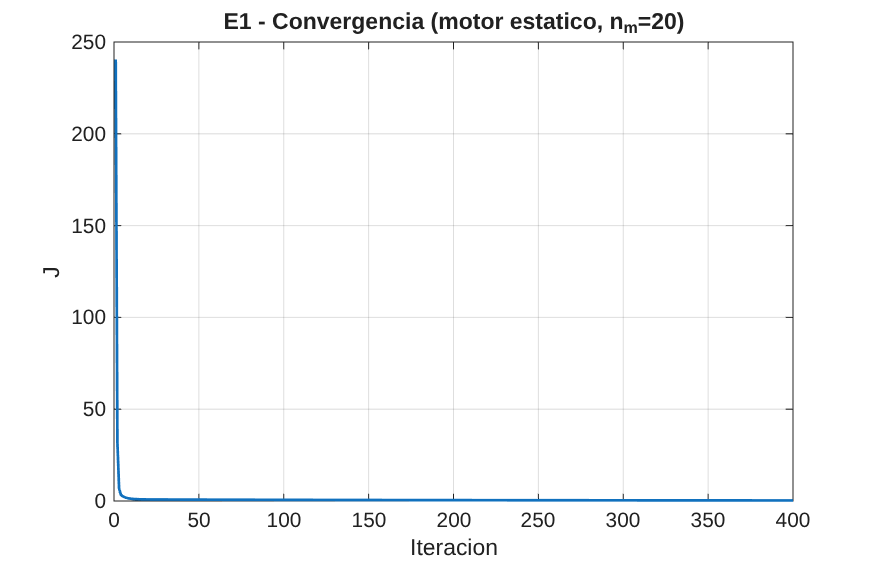
\includegraphics[width=\linewidth]{figs/E1_conv.png}
  \caption{Convergencia del costo $J$ (modelo estático, $n_m=20$).}
  \label{fig:E1conv}
\end{minipage}\hfill
\begin{minipage}{0.48\linewidth}\centering
  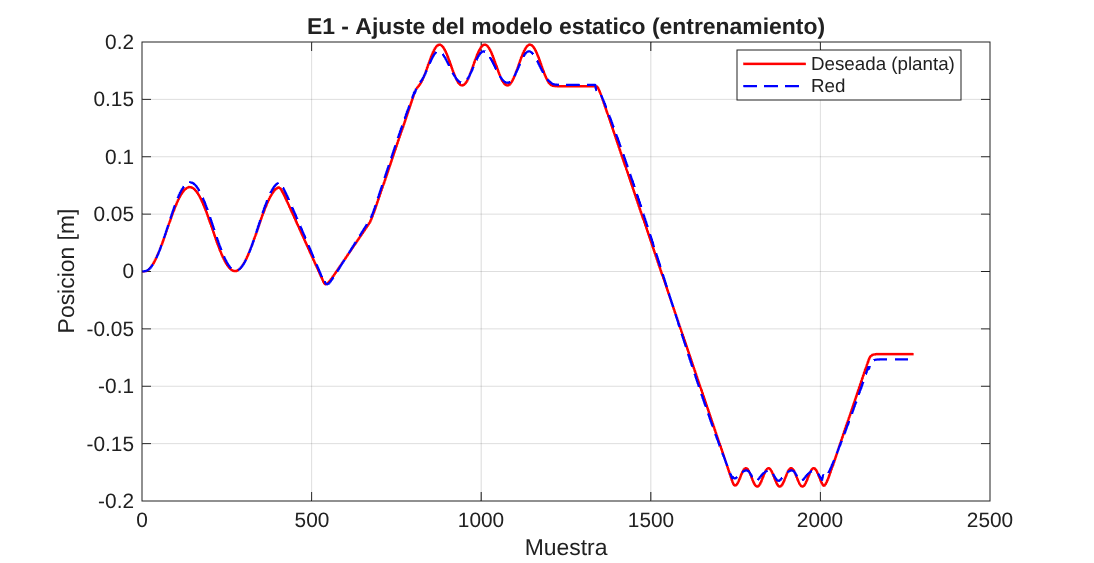
\includegraphics[width=\linewidth]{figs/E1_fit.png}
  \caption{Ajuste del modelo estático sobre los datos de entrenamiento.}
  \label{fig:E1fit}
\end{minipage}
\end{figure}

\paragraph{Influencia del ruido de medición.}
Como la red usa posiciones \emph{medidas} pasadas como entradas, el ruido de medición
degrada el modelo de forma directa. La Fig.~\ref{fig:E1noise} muestra que el RMSE
(en unidades físicas, frente a la señal limpia) crece de $\approx 0.003$~m sin ruido a
$\approx 0.038$~m con $\eta=0.1$: un aumento de más de $10\times$. El ruido entra
tanto por el objetivo como por los regresores, por lo que el modelo estático nunca se
independiza de él.

\paragraph{Número de neuronas y de regresores.}
La Tabla~\ref{tab:E1} resume ambos barridos. Aumentar $n_m$ reduce el error de ajuste
(de $3.0\%$ con 3 neuronas a $1.3\%$ con 80), como cabe esperar por la mayor capacidad
de la red (Fig.~\ref{fig:E1neurons}). En cambio, para esta planta casi lineal, agregar
más posiciones pasadas \emph{no} mejora el ajuste a iteraciones fijas: con un solo
retardo el error es el menor ($0.8\%$) y crece al añadir regresores
(Fig.~\ref{fig:E1regressors}), porque los parámetros adicionales ralentizan la
convergencia sin aportar información dinámica nueva. La Fig.~\ref{fig:E1eta} confirma
el compromiso habitual de la tasa de aprendizaje: $\eta$ pequeño converge lento y
$\eta$ grande converge rápido pero con riesgo de oscilación.

\begin{table}[H]
\centering
\caption{Error relativo de ajuste del modelo estático.}
\label{tab:E1}
\begin{tabular}{lcccccc}
\toprule
Neuronas $n_m$ & 3 & 5 & 10 & 20 & 40 & 80 \\
Error rel. & 0.030 & 0.029 & 0.021 & 0.026 & 0.024 & 0.013 \\
\midrule
Regresores (\# retardos) & 1 & 2 & 3 & 6 & & \\
Error rel. & 0.008 & 0.013 & 0.013 & 0.026 & & \\
\bottomrule
\end{tabular}
\end{table}

\begin{figure}[H]
\centering
\begin{minipage}{0.32\linewidth}\centering
  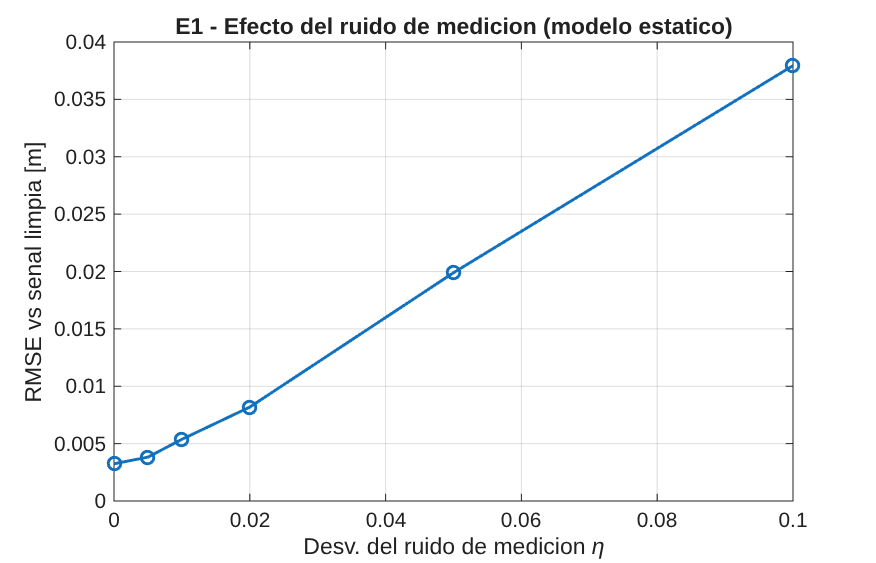
\includegraphics[width=\linewidth]{figs/E1_noise.png}
  \caption{Efecto del ruido.}
  \label{fig:E1noise}
\end{minipage}\hfill
\begin{minipage}{0.32\linewidth}\centering
  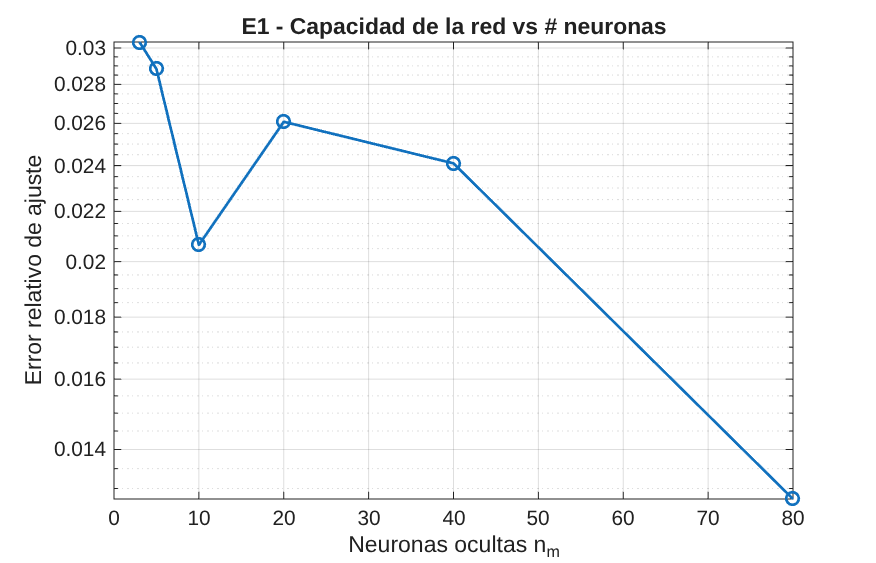
\includegraphics[width=\linewidth]{figs/E1_neurons.png}
  \caption{Error vs $n_m$.}
  \label{fig:E1neurons}
\end{minipage}\hfill
\begin{minipage}{0.32\linewidth}\centering
  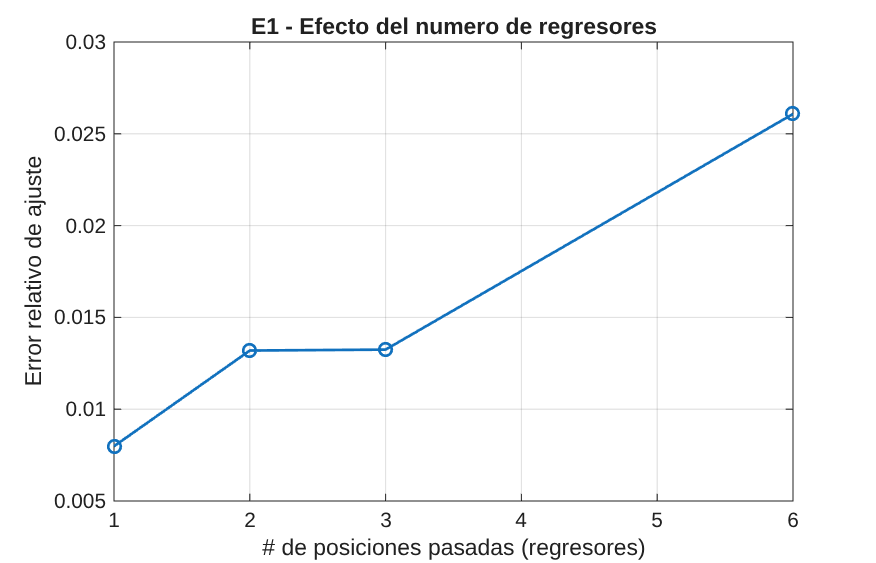
\includegraphics[width=\linewidth]{figs/E1_regressors.png}
  \caption{Error vs \# regresores.}
  \label{fig:E1regressors}
\end{minipage}
\end{figure}

\begin{figure}[H]
\centering
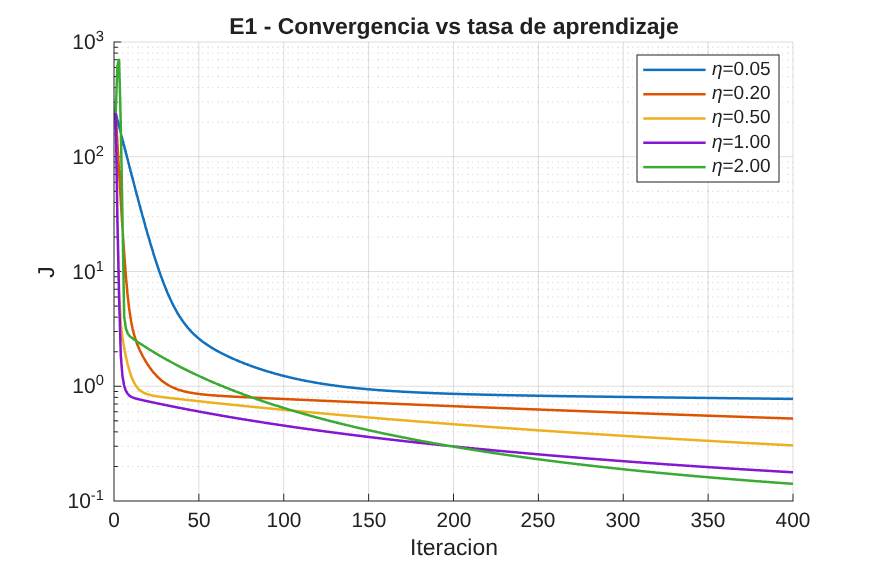
\includegraphics[width=0.55\linewidth]{figs/E1_eta.png}
\caption{Convergencia del costo para distintas tasas de aprendizaje $\eta$.}
\label{fig:E1eta}
\end{figure}

\subsection{Modelo dinámico DBP (2 estados)}
\label{sec:E2}

Se entrenó la red recurrente sobre la planta no lineal ($nm=50$, $\eta=0.05$).
El error relativo total cae hasta $\approx 8.6\%$ (Fig.~\ref{fig:E2conv}) y el modelo,
ejecutado en \textbf{lazo cerrado} (simulación libre, sin realimentar la señal real),
sigue ambos estados $z_1,z_2$ de la planta (Fig.~\ref{fig:E2fit}). Esto es notable:
el modelo genera su propia trayectoria a partir solo de la entrada $u$.

\begin{figure}[H]
\centering
\begin{minipage}{0.44\linewidth}\centering
  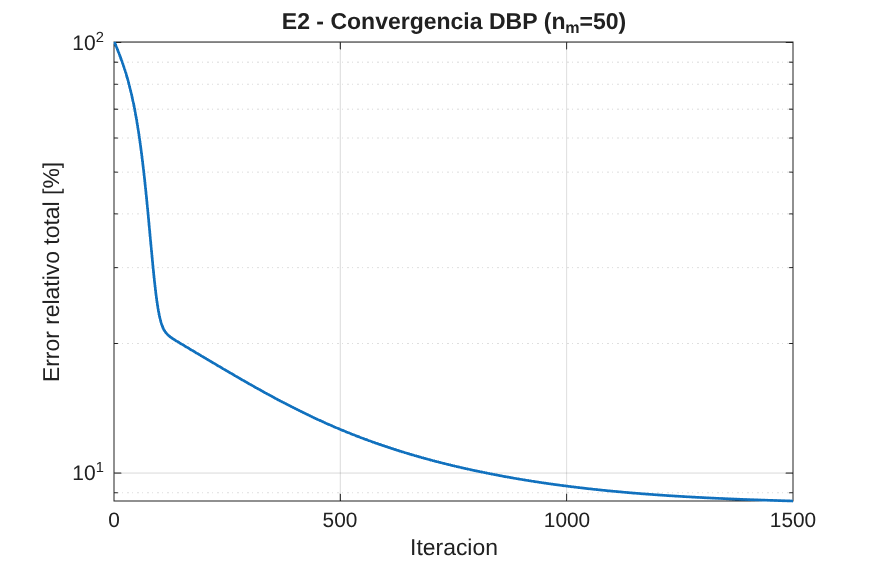
\includegraphics[width=\linewidth]{figs/E2_conv.png}
  \caption{Convergencia del error relativo (DBP).}
  \label{fig:E2conv}
\end{minipage}\hfill
\begin{minipage}{0.54\linewidth}\centering
  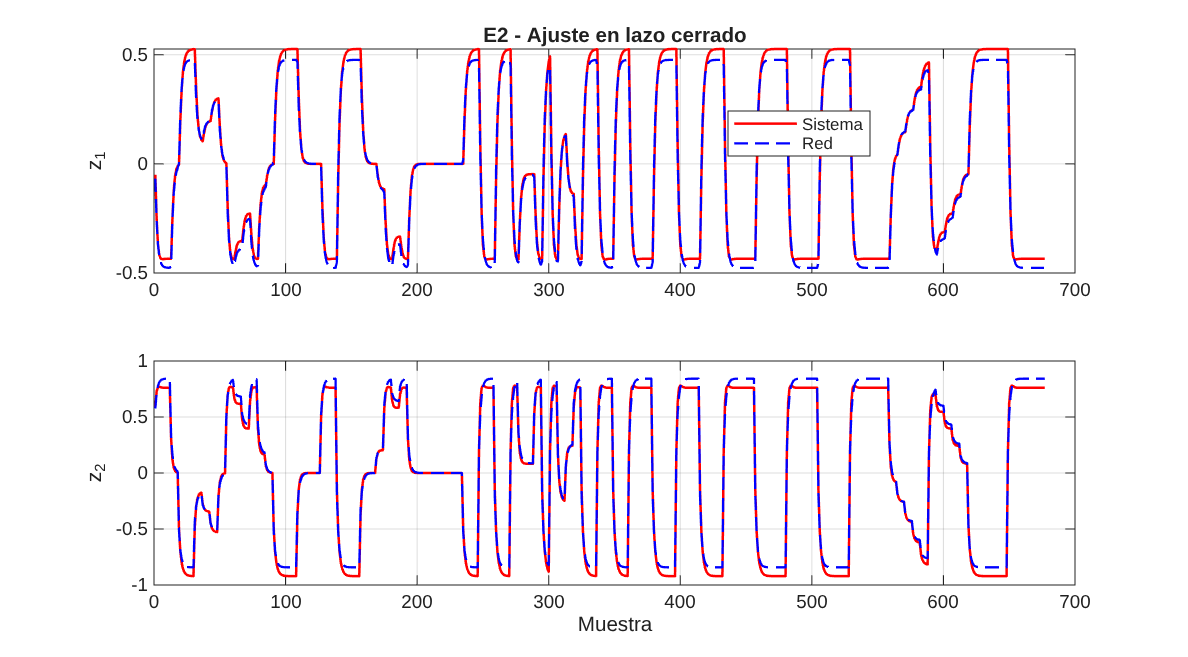
\includegraphics[width=\linewidth]{figs/E2_fit.png}
  \caption{Ajuste en lazo cerrado de $z_1$ y $z_2$.}
  \label{fig:E2fit}
\end{minipage}
\end{figure}

\paragraph{Medición parcial (matriz $Q$).}
Con $q=[1;1]$ se miden ambos estados y el RMSE en lazo cerrado es
$[0.067,\,0.060]$. Con $q=[1;0]$ (solo se mide $z_1$), el estado no medido $z_2$
queda esencialmente sin observar y su RMSE se dispara a $0.68$, arrastrando también
a $z_1$ ($0.16$) —Fig.~\ref{fig:E2partial}. Es decir: si un estado no se penaliza en
el costo, el modelo no tiene incentivo para reproducirlo.

\paragraph{Neuronas y tipo de activación.}
El error final disminuye al aumentar $n_m$ (Fig.~\ref{fig:E2neurons}). Por otro lado,
como el término no lineal $0.1\,z_1 u$ es débil frente a $0.5\,u$, una red de
\textbf{neuronas lineales} alcanza casi el mismo error que la sigmoidal
($8.6\%$ en ambos casos, Fig.~\ref{fig:E2act}): la planta es ``casi lineal'' y no
exige la capacidad no lineal de la sigmoide.

\begin{figure}[H]
\centering
\begin{minipage}{0.32\linewidth}\centering
  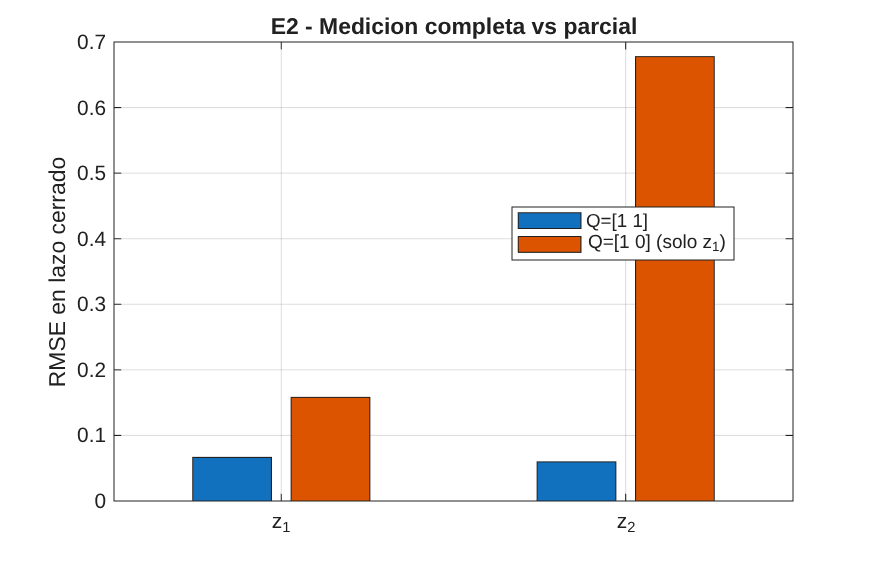
\includegraphics[width=\linewidth]{figs/E2_partial.png}
  \caption{Medición completa vs parcial.}
  \label{fig:E2partial}
\end{minipage}\hfill
\begin{minipage}{0.32\linewidth}\centering
  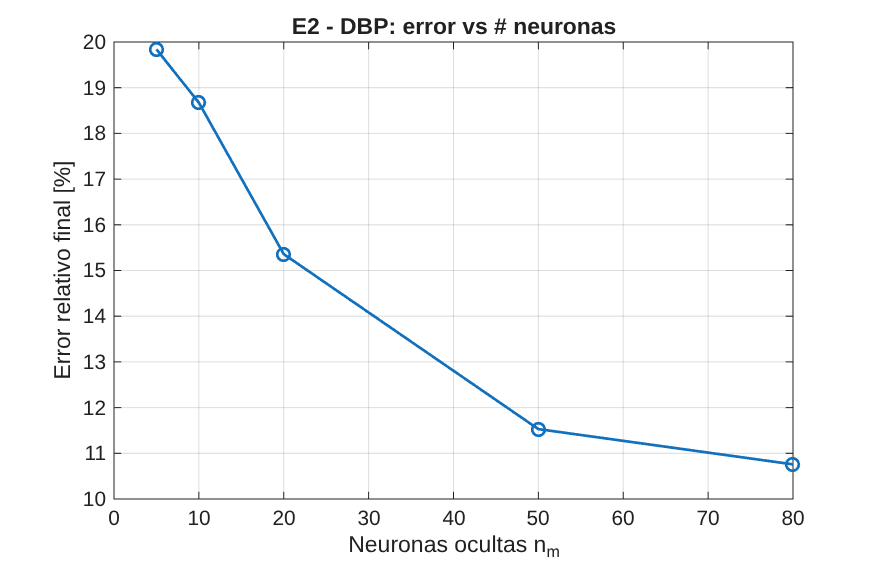
\includegraphics[width=\linewidth]{figs/E2_neurons.png}
  \caption{Error vs $n_m$.}
  \label{fig:E2neurons}
\end{minipage}\hfill
\begin{minipage}{0.32\linewidth}\centering
  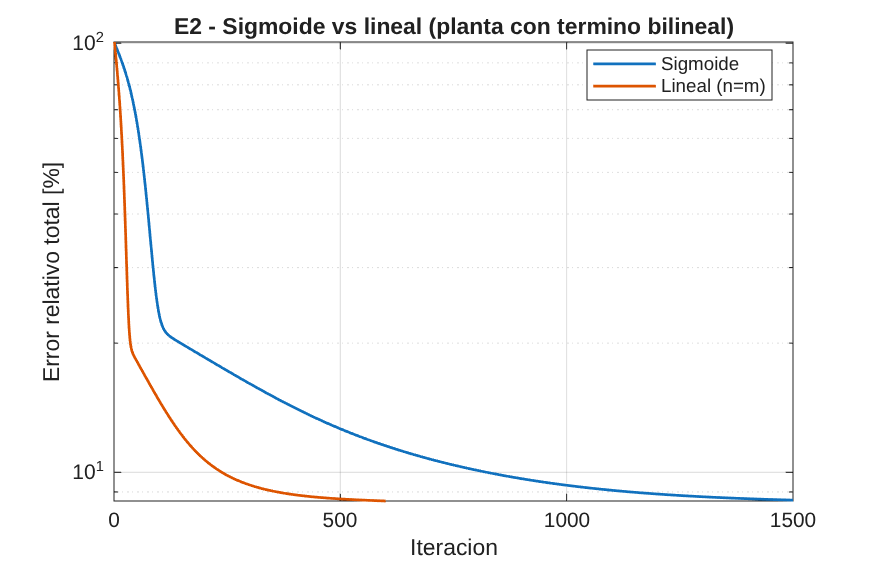
\includegraphics[width=\linewidth]{figs/E2_activation.png}
  \caption{Sigmoide vs lineal.}
  \label{fig:E2act}
\end{minipage}
\end{figure}

\subsection{Estático vs dinámico ante ruido de medición}
\label{sec:E3}

Este es el experimento central. Sobre la \emph{misma} planta no lineal se entrenan
ambos modelos con datos de salida \textbf{contaminados por ruido} de desviación $\eta$,
y se mide su error frente a la señal limpia. La diferencia clave está en el modo de
operación: el modelo estático se evalúa en su uso nativo (predicción a un paso,
alimentado con la salida \emph{medida} ruidosa), mientras que el dinámico se evalúa en
\textbf{lazo cerrado}, donde no vuelve a usar la medición.

\begin{table}[H]
\centering
\caption{RMSE del modelo frente a la señal limpia, según el ruido de medición $\eta$.}
\label{tab:E3}
\begin{tabular}{lcccccc}
\toprule
$\eta$ & 0 & 0.01 & 0.02 & 0.05 & 0.10 & 0.15 \\
\midrule
Estático (1 paso) & 0.022 & 0.023 & 0.026 & 0.032 & 0.040 & 0.048 \\
Dinámico (lazo cerrado) & 0.053 & 0.053 & 0.053 & 0.053 & 0.054 & 0.054 \\
\bottomrule
\end{tabular}
\end{table}

La Fig.~\ref{fig:E3rob}(a) muestra el error absoluto y (b) el error \emph{normalizado}
a su valor sin ruido. El resultado confirma la propiedad esperada: el error del modelo
estático \textbf{crece $\approx 2.15\times$} al pasar de $\eta=0$ a $\eta=0.15$, porque
la medición ruidosa entra directamente por sus entradas y se propaga a la salida. El
modelo dinámico, en cambio, permanece \textbf{prácticamente plano}: una vez entrenado,
es independiente de la señal medida (genera su propia trayectoria), por lo que el ruido
solo lo afectó durante el entrenamiento y allí se promedió. La Fig.~\ref{fig:E3traces}
lo ilustra: con $\eta=0.1$, la salida del modelo dinámico ``filtra'' el ruido y sigue
la señal limpia, no la ruidosa.

\begin{figure}[H]
\centering
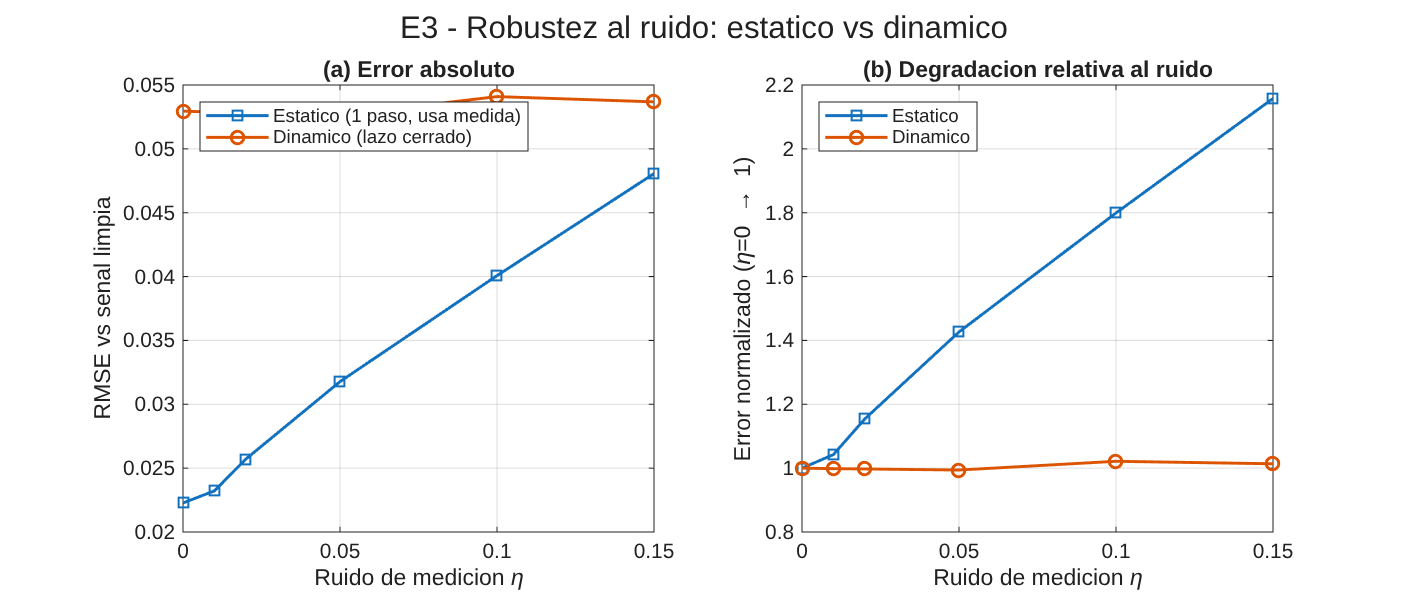
\includegraphics[width=0.95\linewidth]{figs/E3_noise_robustness.png}
\caption{Robustez al ruido de medición. (a) RMSE absoluto; (b) degradación relativa
(cada curva normalizada a su error con $\eta=0$).}
\label{fig:E3rob}
\end{figure}

\begin{figure}[H]
\centering
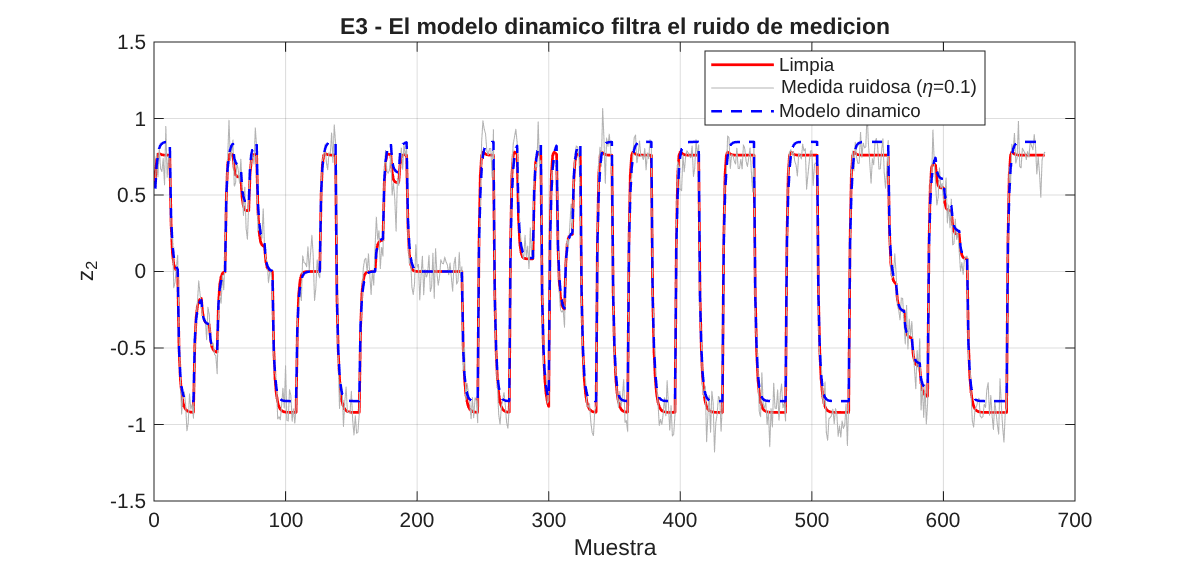
\includegraphics[width=0.7\linewidth]{figs/E3_traces.png}
\caption{Con $\eta=0.1$, el modelo dinámico reproduce la señal limpia y descarta el
ruido de medición.}
\label{fig:E3traces}
\end{figure}

Nótese que, en términos absolutos, el modelo estático a un paso arranca con menor error
(tarea más sencilla que la simulación libre); lo relevante aquí es la \emph{tendencia}:
el estático se degrada de forma monótona con el ruido y el dinámico no.

\subsection{Identificación de parámetros de un sistema lineal}
\label{sec:E4}

Se identificó el sistema lineal $y_{k+1}=Ay_k+Bu_k$ con
$A=\left[\begin{smallmatrix}0.6&0.8\\0.3&-0.1\end{smallmatrix}\right]$,
$B=\left[\begin{smallmatrix}0\\-0.2\end{smallmatrix}\right]$, entrenando la red lineal de
una capa (Sec.~\ref{sec:codeE4}). Se compararon los dos modos de entrenamiento
(Fig.~\ref{fig:E4conv}): el de \emph{lazo cerrado} del script original (error de salida)
y el de \emph{forzado con el estado medido} (error de ecuación, alimentando el estado medido).

Con forzado con el estado medido y entrada rica, la red \textbf{recupera exactamente} los parámetros
(error $\|v-v_{\text{true}}\|_F \approx 2.5\times10^{-8}$):
\[
  v = \begin{bmatrix}0.600 & 0.300\\ 0.800 & -0.100\\ 0.000 & -0.200\end{bmatrix}
  \;=\;\begin{bmatrix}A^{\top}\\ B^{\top}\end{bmatrix}\; \text{(exacto).}
\]
En cambio, el modo de lazo cerrado del script queda en un error de $0.234$: la
optimización de error de salida es no convexa y más difícil, lo que explica por qué el
script original recurre al \emph{arranque desde pesos previos} (\code{load zz1v}).

\paragraph{Riqueza de la entrada.}
La identificabilidad depende críticamente de que la entrada excite todos los modos.
Con la señal rica multinivel el error de parámetros es prácticamente nulo, mientras que
con un escalón o una senoidal única sube a $\sim 5\times10^{-1}$
(Fig.~\ref{fig:E4rich}): una entrada pobre no aporta información suficiente para
determinar $A$ y $B$.

\paragraph{Ruido de medición.}
El ruido introduce un \textbf{sesgo creciente} en los parámetros identificados
(Fig.~\ref{fig:E4noise}): al usar la salida medida (ruidosa) como regresor, el estimador
de mínimos cuadrados se sesga (por el ruido presente en los regresores), y
$\|v-v_{\text{true}}\|_F$ crece de forma monótona con $\eta$.

\begin{figure}[H]
\centering
\begin{minipage}{0.33\linewidth}\centering
  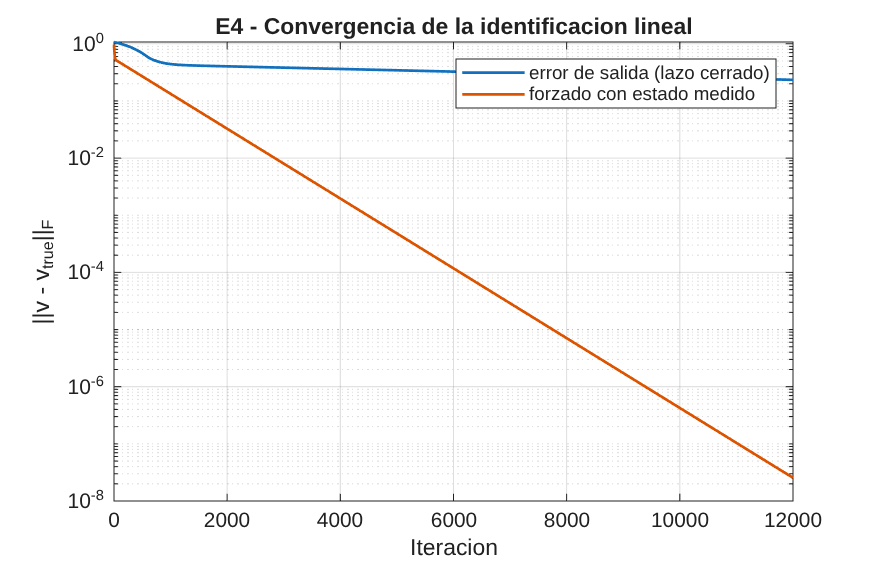
\includegraphics[width=\linewidth]{figs/E4_conv.png}
  \caption{Convergencia: lazo cerrado vs forzado con el estado medido.}
  \label{fig:E4conv}
\end{minipage}\hfill
\begin{minipage}{0.33\linewidth}\centering
  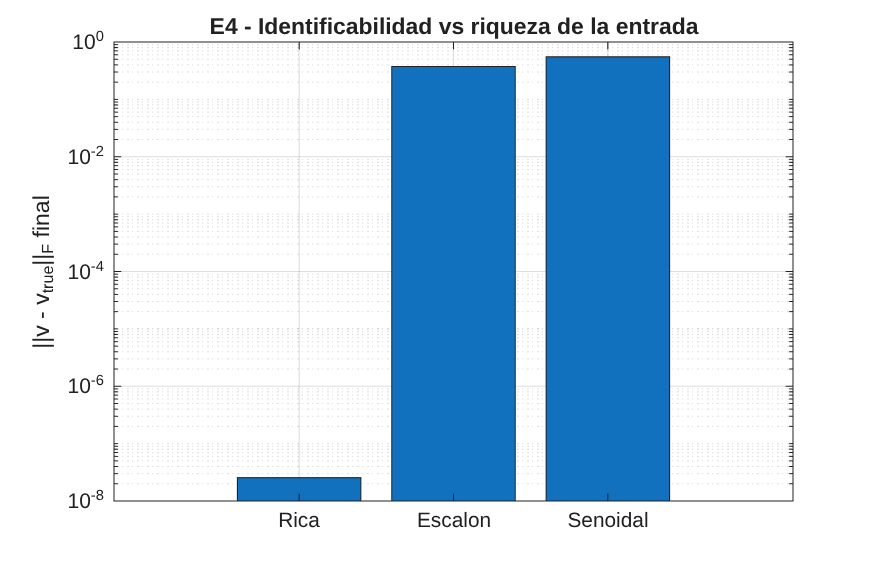
\includegraphics[width=\linewidth]{figs/E4_richness.png}
  \caption{Error vs riqueza de la entrada.}
  \label{fig:E4rich}
\end{minipage}\hfill
\begin{minipage}{0.33\linewidth}\centering
  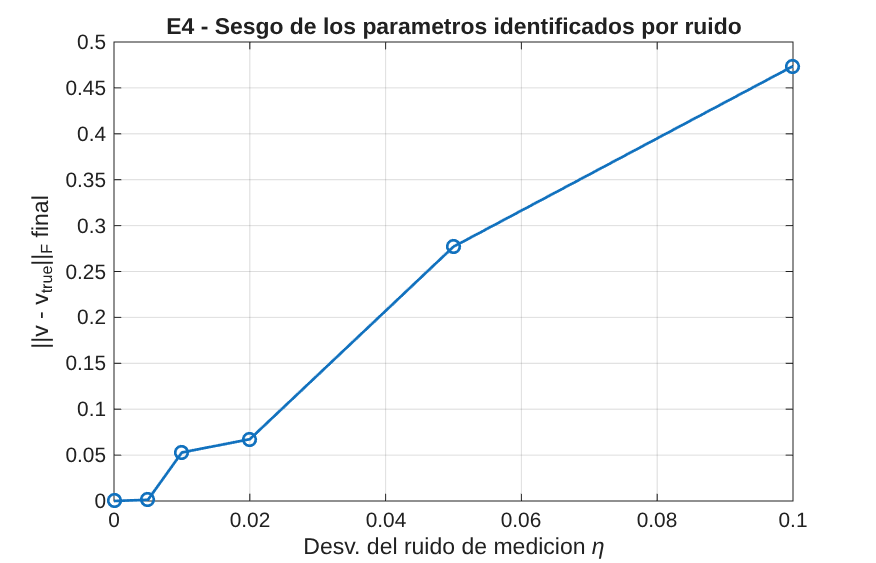
\includegraphics[width=\linewidth]{figs/E4_noise.png}
  \caption{Sesgo por ruido de medición.}
  \label{fig:E4noise}
\end{minipage}
\end{figure}

\subsection{Arquitecturas: una vs dos capas y sistema de 3 variables}
\label{sec:E56}

\paragraph{Una vs dos capas ocultas.}
Sobre la misma planta no lineal se comparó la red DBP de \textbf{una} capa oculta
(12 neuronas) con la de \textbf{dos} capas (12--10). A igualdad de iteraciones, la red
de una capa alcanzó un error final de $17.9\%$ frente al $22.7\%$ de la de dos capas
(Fig.~\ref{fig:E5}). Añadir una segunda capa \emph{no} mejoró el resultado: aumenta el
número de parámetros y la profundidad de la regla de la cadena (dos sigmoides en la
recursión), lo que hace el entrenamiento más lento y con gradientes más difíciles de
propagar. Para una planta de baja complejidad, una sola capa es suficiente y preferible.

\paragraph{Sistema de 3 variables.}
El DBP escala directamente a un sistema de 3 salidas (Jacobiano $3\times3$). El modelo
lineal recurrente ajustó las tres variables con un error relativo de solo $1.7\%$
(Fig.~\ref{fig:E6}), confirmando que la metodología es general en el número de estados.

\begin{figure}[H]
\centering
\begin{minipage}{0.46\linewidth}\centering
  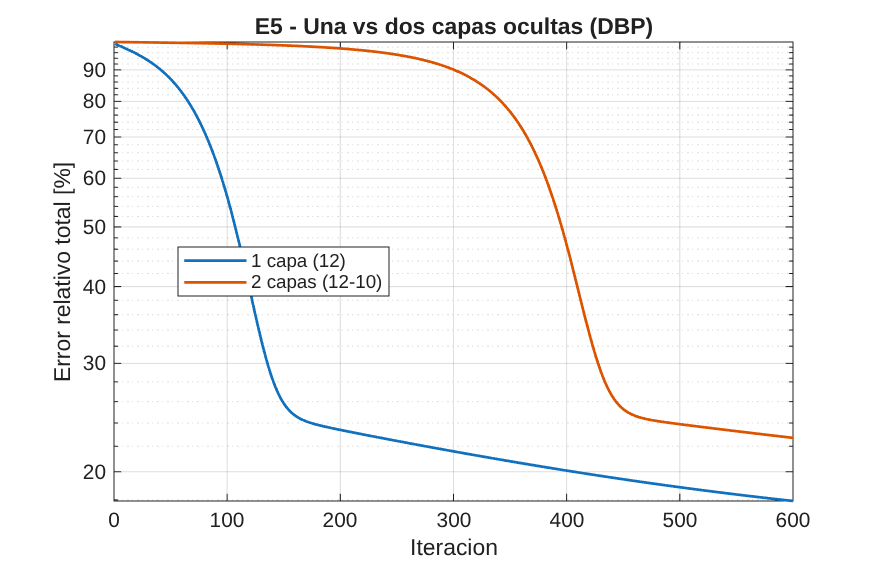
\includegraphics[width=\linewidth]{figs/E5_layers.png}
  \caption{Convergencia: una vs dos capas ocultas.}
  \label{fig:E5}
\end{minipage}\hfill
\begin{minipage}{0.52\linewidth}\centering
  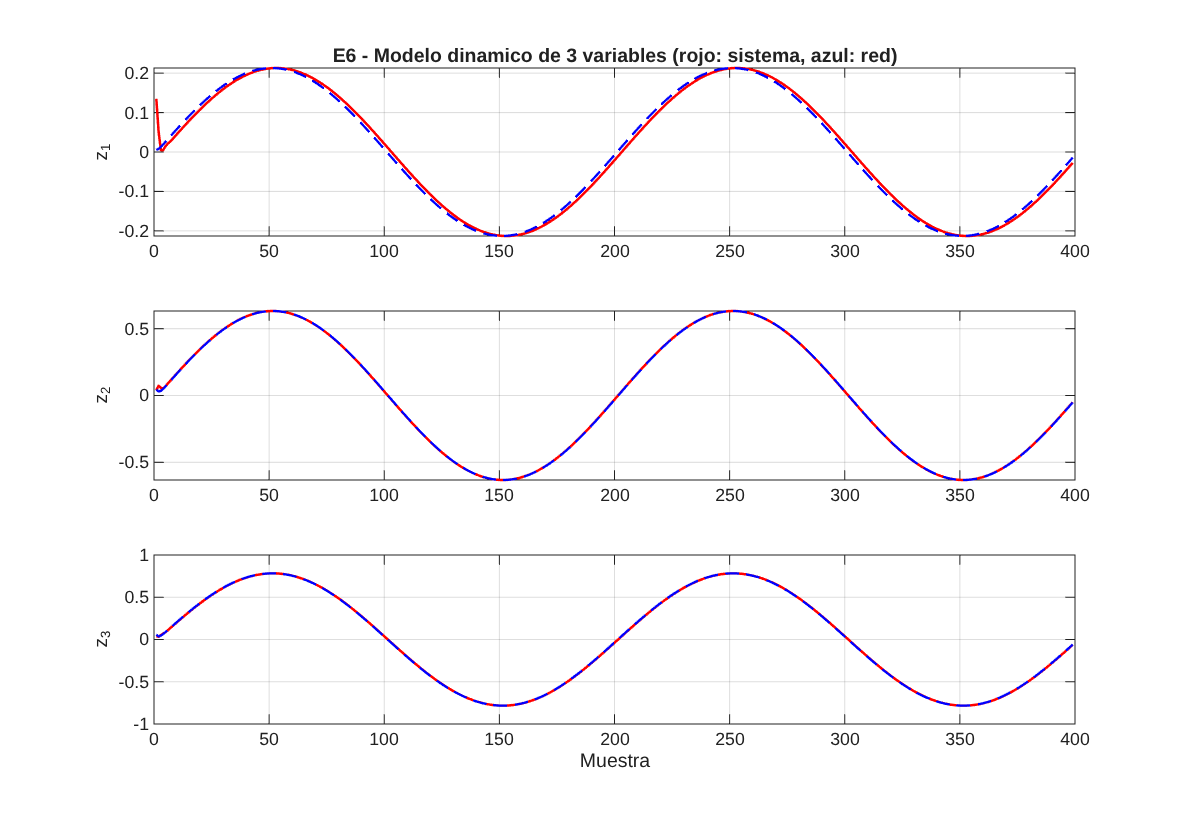
\includegraphics[width=\linewidth]{figs/E6_three.png}
  \caption{Modelo dinámico de un sistema de 3 variables.}
  \label{fig:E6}
\end{minipage}
\end{figure}

% ================= CONCLUSIONES =================
\section{Conclusiones}

\begin{enumerate}
  \item \textbf{Ambos enfoques modelan la dinámica}, pero por vías distintas: el modelo
  estático la reconstruye con regresores (entradas y salidas pasadas medidas) y
  \emph{retropropagación} clásica; el dinámico la incorpora en la propia recurrencia y se
  entrena con DBP, propagando las derivadas totales a través del Jacobiano de la red.

  \item \textbf{El ruido de medición separa claramente a las dos familias}
  (Sec.~\ref{sec:E3}). El modelo estático usa la salida medida como entrada también en
  operación, por lo que su error crece de forma monótona con el ruido ($\approx 2.15\times$
  entre $\eta=0$ y $\eta=0.15$). El modelo dinámico, tras el entrenamiento, es
  independiente de la señal medida y su error en lazo cerrado permanece esencialmente
  constante: filtra el ruido. Este es el argumento principal a favor del modelo dinámico
  cuando se lo usa como simulador.

  \item \textbf{Los parámetros de diseño influyen de forma consistente}: más neuronas
  reducen el error de ajuste (E1, E2); una tasa de aprendizaje $\eta$ mayor acelera la
  convergencia a costa de estabilidad (E1); y penalizar en el costo un estado que no se
  mide (matriz $Q$ con un cero) hace que ese estado quede sin reproducir (E2).

  \item \textbf{Complejidad adecuada al problema}: para plantas casi lineales, una red de
  neuronas lineales iguala a la sigmoidal (E2) y una sola capa oculta supera a dos capas
  (E5). Más capacidad no siempre es mejor a iteraciones fijas.

  \item \textbf{La red lineal identifica los parámetros del sistema} (E4): sus pesos
  \emph{son} las matrices $A$ y $B$. La identificación es limpia cuando se dispone del
  estado medido (formulación de \emph{error de ecuación}, convexa) y requiere una entrada
  \textbf{rica} para ser identificable; una señal pobre (escalón o senoidal única) no
  excita todos los modos y deja parámetros mal estimados. El ruido de medición introduce
  un sesgo creciente en los parámetros identificados. La variante en lazo cerrado del
  script original (error de salida) es más difícil de optimizar, lo que justifica el
  \emph{arranque desde pesos previos} (\code{load zz1v}) que emplea.
\end{enumerate}

\appendix
\section{Archivos del proyecto}
Los experimentos se generan ejecutando \code{Informe/exp/run\_all.m} en MATLAB. Las
rutinas de entrenamiento reutilizables son \code{lib\_static.m} (estático) y
\code{lib\_dbp.m} (dinámico, DBP vectorizado para $ns$ salidas). Cada experimento
E1--E6 tiene su propio script y guarda sus figuras en \code{Informe/figs/} y sus
métricas en \code{*\_metrics.mat}.

\end{document}
